\documentclass[11pt]{article}
\usepackage{geometry}
\usepackage{graphicx}
\usepackage{enumitem}
\usepackage{float}
\usepackage{amsmath}

\geometry{a4paper, top=0.5in, bottom=0.5in, right=0.75in, left=0.75in}

\title{CDC}
\author{Abanoub Emad Hanna}
\date{}

\begin{document}

\maketitle

\section*{Metastability}
\subsection*{Causes}
Metastability occurs when input changes during aperture time. This might happen due to:
\begin{itemize}
    \item 
    \textbf{Asynchronous inputs}
    \item \textbf{Clock Domain Crossing (CDC):} Two clocks can be considered different domains or 'Asynchronous' if they are \textbf{not from the same source} even if they have same frequency. If the 2 clocks have tha same frequency, despite the fact that the phase difference will be constant during the operation of the system, after each startup the phase difference is different each time.
\end{itemize}

\subsection*{Explanation}
\begin{minipage}[t]{0.6\textwidth}
    \vspace*{-95pt}
    Transitioning during the aperture window causes the master's latch to close while having \(\Delta V_{in} (V_x - V_y)\) around $V_m$.\\
    FF's output will not settle before \(t_{pcq}\), since latch's delay is variable given by:
    \[
        t_d = \tau \ln\frac{V_{DD}}{\Delta V_{in}}, \text{ where } \tau=\frac{C_L}{g_m}
    \]
\end{minipage}%
\hfill
\begin{minipage}[t]{0.35\textwidth}
    \centering
    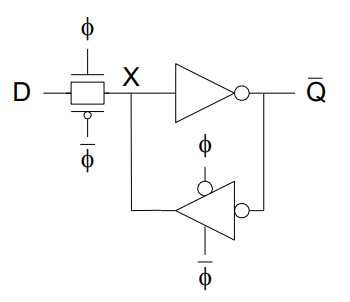
\includegraphics[scale=0.55]{1.png}
\end{minipage}

\subsection*{Effects}
\begin{enumerate}
    \item \textbf{High CLK-to-Q Delay:} This might lead to setup time violation for the receiver FF.
    \item \textbf{Short Circuit Current:} Since $\Delta V_{in}$ is around $V_m$, the short circuit current is high.
    \item \textbf{Different Values Propagation:} If the metastable FF drives 2 paths, the 2 paths might have different values.
\end{enumerate}

\subsection*{Probability}
\begin{itemize}
    \item The probability of metastability per input change is given by ($T_a=t_{setup}+t_{hold}$): 
    \begin{equation*}
        P(MS)=\frac{T_a}{T_c}=T_af_c
    \end{equation*}
    \item Fialure Rate = BER = Probability of failure per second is given by:
    \begin{equation*}
        FR = f_{in}\frac{T_a}{T_c}=T_af_cf_{in}
    \end{equation*}
    \item Mean Time Between Failure (MTTF) is given by:
    \begin{equation*}
        MTBF = \frac{1}{FR} = \frac{1}{T_af_cf_{in}}
    \end{equation*}
\end{itemize}
\textbf{Note:} Metastability can never be eliminated, but it can be minimized.
\pagebreak

\section*{Synchronization}

\subsection*{Simple Bit Synchronization}

\subsubsection*{Behaviour}
\begin{itemize}
    \item If $\Delta V_{in}$ is exactly $V_m$, the output should theoritically be stuck at $V_m$ (review inverter curve). However, presence of noise as well as mismatch between inverters' switching thresholds would make it $V_m + \Delta$, so the output will be driven to $V_{DD}$ or GND in the same clock cycle due to the high gain of the inverters in the FF.
    \item However, this value might be wrong, but the FF will eventually settle to the correct value after an unkonwn number of clock cycles (2 or 3 for double flop synchronizer) depending on the $\Delta$ around $V_m$.
    \item Therefore, the input should be stable for at least $1.5*T_{clk}$ of the receiver clock to ensure correct data sampling.
\end{itemize}
\textbf{Notes:}
\begin{itemize}
    \item If the difference in clock speeds is huge, a third FF is added.
    \item Some librarirs provide synchronizer cells called meta-hardened flops.
    \item $t_{resolve}=T_{clk}-t_{setup}$
\end{itemize}

\begin{center}
    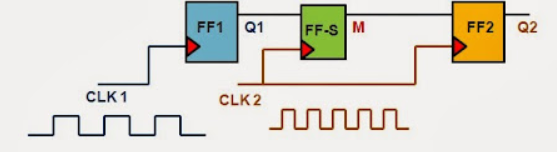
\includegraphics[scale=0.6]{2.png}
\end{center}

\subsubsection*{Probability}
\begin{itemize}
    \item Probability of synchronizer failure is given by:
        \begin{equation*}
            P(sync failure) = \frac{\Delta V_{in}}{V_{DD}} = \exp\left(-\frac{t_{resolve}}{\tau}\right)
        \end{equation*}
    \item Probability of system failure is given by:
        \begin{equation*}
            P(system failure) = P(MS)P(sync failure) = T_af_c\exp\left(-\frac{t_{resolve}}{\tau}\right)
        \end{equation*}
    \item Mean Time Between Failure (MTBF) is given by:
        \begin{equation*}
            MTBF = \frac{1}{T_af_cf_{in}\exp\left(-\frac{t_{resolve}}{\tau}\right)}
        \end{equation*}
\end{itemize}



\subsection*{Pitfalls}
\begin{itemize}
    \item Do NOT synchronize data lines.
    \item Do NOT drive two synchronizers with the same signal; The two synchronizers can resolve to different values.
    \item Do NOT put the sync FFs far apart or put logic between them; The wire or logic delay will eat from your resolution time.
    \item Synchronizers must have good feedback loops; You cannot use dynamic FFs
\end{itemize}

\subsection*{Data Bus Synchronization}
Simple bit synchronizer can not be used for bus synchronization, due to \textbf{Different Routing Delays}. Different bits might arrive at different times during the aperture time causing each FF to have different $\Delta V_{in}$, so each FF might rseolve metastability at different clock cycles, so some bits would have an old value, while others have a new one.

\subsubsection*{Gray Coding Technique}
\begin{itemize}
    \item Gray coding ensures that only one bit changes at a time, so the non-changing bits don't care if value is old or new since they are the same.
    \item It is only used for data that follows a certain pattern (e.g. counter).
\end{itemize}

\subsubsection*{Enable-Based Technique}
\begin{itemize}
    \item Source domain sends an enable signal, which is synchronized by two FFs.
    \item Data should be constant for 2 cycles, so it is sampled correctly by the receiver.
    \item The data receiving FFs don't suffer from metastability, since they are only enabled when the data is stable.
    \item Instead of using FFs that have EN, a MUX can be used to select between the old and new values.
\end{itemize}
\begin{center}
    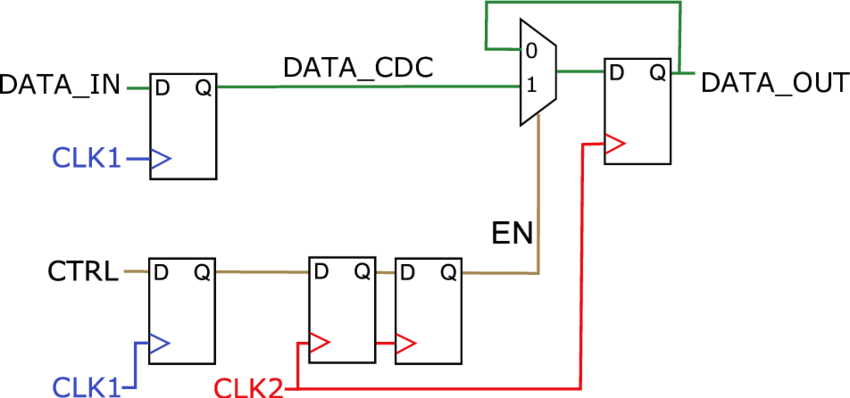
\includegraphics[scale=0.25]{3.png}
\end{center}

\subsubsection*{Handshake Technique}
\begin{itemize}
    \item Source domain sends a request signal, which is synchronized by two FFs.
    \item The receiver domain sends an acknowledge signal, which is also synchronized by two FFs.
    \item This technique is preferred when data is sent occasionally between subsystems, due to its very high latency.
    \item Handshake protocol can be:
    \begin{itemize}
        \item \textbf{4-Phase:} Request and Acknowledge are level sensitive.
        \item \textbf{2-Phase:} Request and Acknowledge are edge sensitive.
    \end{itemize}
    \item Pulse to edge and edge to pulse converters are used to convert between the two protocols.
\end{itemize}
\begin{center}
    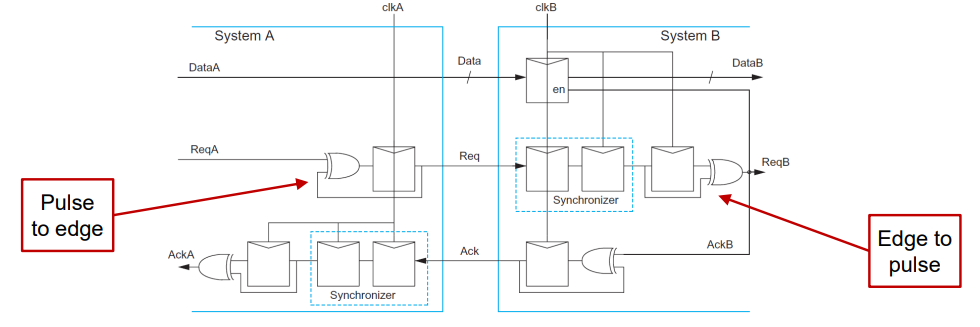
\includegraphics[scale=0.7]{4.png}
\end{center}
\textbf{Note:} Only fast to slow domain crossing causes data loss.

\pagebreak

\subsection*{Asynchronous FIFO}
FIFO is best suited when transmitter is faster than receiver, since it can store data until the receiver is ready to read it. 
\subsubsection*{Operation}
\begin{itemize}
    \item \textbf{Empty Flag Condition:} Empty flag is set when read pointer is incremented and the new value is equal to the write pointer. Otherwise, we would have read same value twice.
    \item \textbf{Full Flag Condition:} Full flag is set when write pointer is incremented and the new value is equal to the read pointer. Otherwise, we would have overwritten an unread data.
    \item To differentiate between full and empty flags, an additional bit is added to the pointers.
    \item Comparing the pointers from different domains would lead to metastability, so double flop synchronizers are used. Since pointers are multi-bit, gray coding must be used to avoid data incoherence.
\end{itemize}

\subsubsection*{Conservative Scenarios}
These scenarios happen due to the added latency of the pointers' synchronizers. They are not catastrophic as data is not lost, but operation falsely stops for 1 clock cycle. For example:
\begin{itemize}
    \item When comparing pointers for empty flag, the write pointer could be outdated and equal to read pointer, despite the fact that it has been incremented, so the empty flag is raised until correct value is written.
    \item When comparing pointers for full flag, the read pointer could be outdated and equal to write pointer, despite the fact that it has been incremented, so the full flag is raised until correct value is read.
\end{itemize}
\begin{center}
    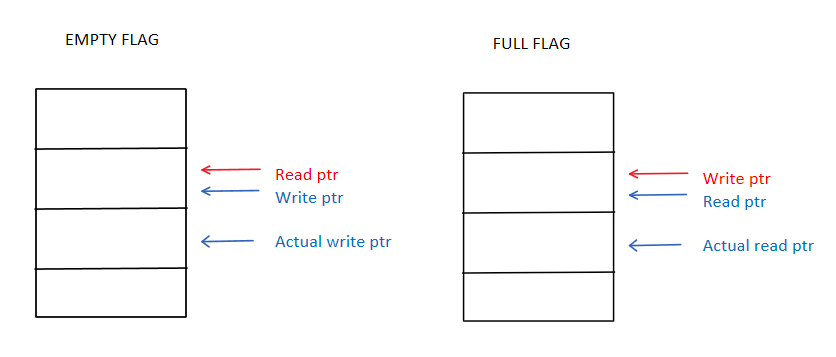
\includegraphics[scale=0.8]{7.png}
\end{center}

\subsubsection*{Depth Calculation}
\textbf{Definitions:} 
\begin{itemize}
    \item \textbf{Effective frequency:} Since there might be constatnt idle cycles during writing and reading, the write/read frequency is reduced. For example, if there is 3 idle clock cycles between successive writes/reads, the effective frequency is $\frac{1}{4}f_{write}$.
    \item \textbf{Burst Length:} Number of data items to be transferred.
\end{itemize}
\textbf{Example:}
\begin{itemize}
    \item \textbf{Givens:} $f_{write}=80MHz$, $f_{read}=50MHz$, Burst Length = 120, Write idle cycles = 1, Read idle cycles = 3.
    \item \textbf{Solution:}
        \begin{itemize}
            \item \textbf{Effective frequencies:} $f_{write}=80/2=40$MHz, $f_{read}=50/4 = 12.5$MHz.
            \item \textbf{Write Time:} $120 * (1/40)=3\mu$s
            \item \textbf{Number of items that can be read:} $3\mu *12.5M=37.5\simeq 37$
            \item \textbf{Remaining data to be stored:} $120-37=83$
            \item Therefore, the FIFO depth should be at least 83.
        \end{itemize}
\end{itemize}

\begin{center}
    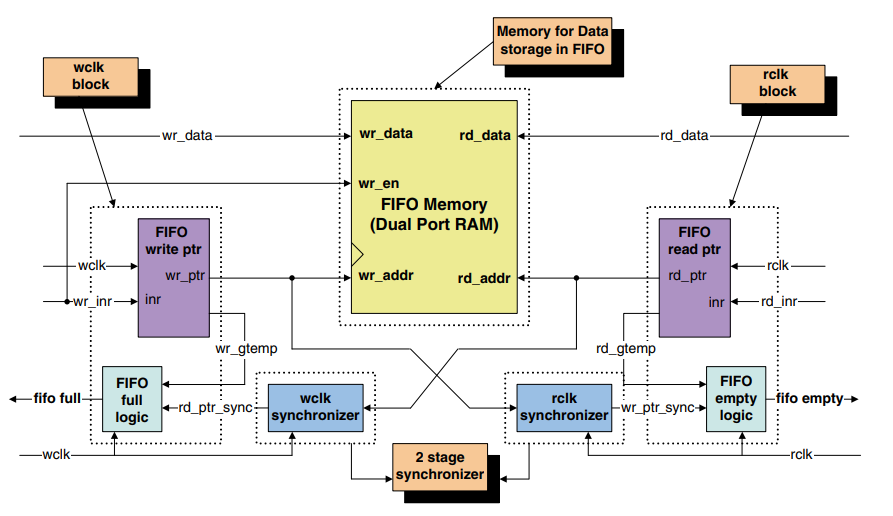
\includegraphics[scale=0.7]{5.png}
\end{center}

\subsection*{Reset Synchronization}
\begin{itemize}
    \item A double flop synchronizer is used to synchronize the reset signal, because reset signal could be de-asserted during the aperture time causing metastability (violating recovery time).
    \item Therefore, designs should have asynchronous reset assertion and synchronous reset de-assertion.
    \item The number of reset synchronizers is equal to number of clock domains.
    \item If Reset signal is not input to second FF, the reset assertion will be synchronous. Also, if there is clock gating, the system will not reset.
\end{itemize}
\begin{center}
    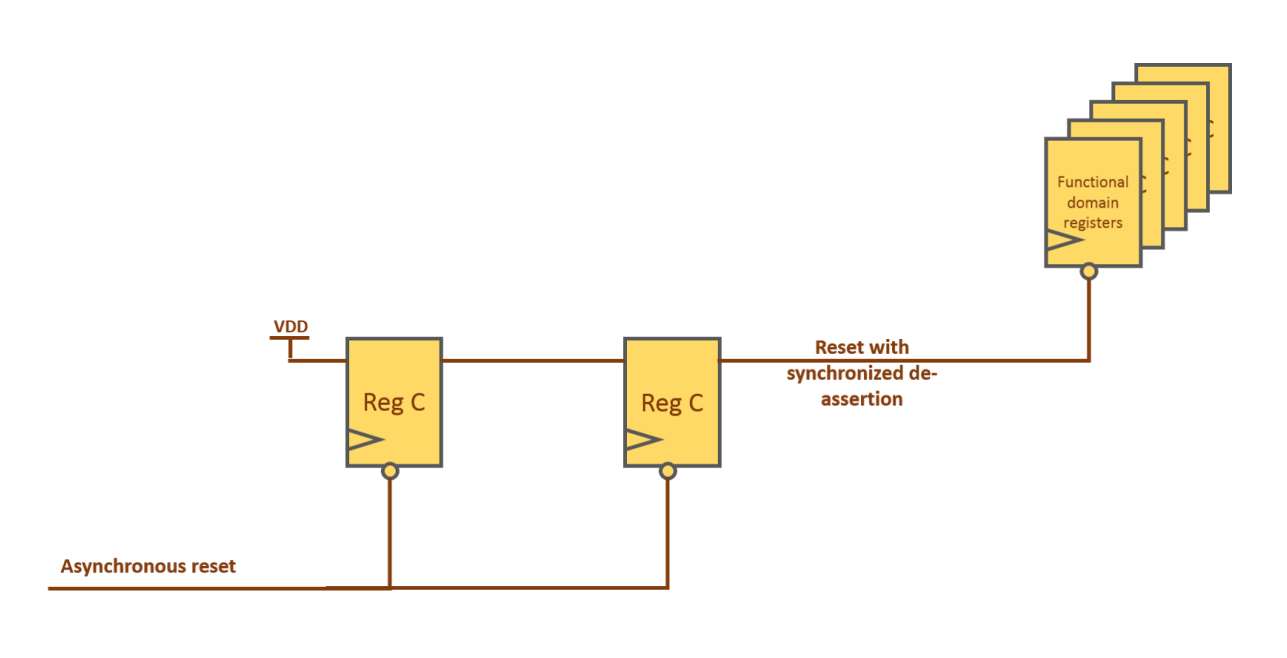
\includegraphics[scale=0.5]{6.png}
\end{center}

\end{document}